\section{File System}


\subsection{Abstractions}

File systems are a very important concept and it makes sense to define an abstract file system. The main task of a file system is to virtualize, this means it should allow for multiplexing, have the same abstraction for multiple file systems implementation.

\subsubsection{Access Control}

We want to enforce some access control for our files. We call user or group of users a \textbf{principal} and files \textbf{objects}. One of the simplest way of representing this information would be in a matrix format. Each row would be a principal and columns correspond to objects. A entry in this matrix describes the rights the principal has in regards to the object. The problem with this idea is that such a matrix would become too large. \medskip

Another idea would be access control lists, a more compact representation. For each file you need to specify user and its access right, so you do not have to save any information on principals that do not have any rights to a file. If a new file gets created we use mandatory access control (MAC) to set the rights to a file. MAC defines the access policy centrally, so the principals cannot make policy decisions. This is easy to implement but hard to customize if you need special permissions. \medskip

A third idea would be to use capabilities, this means that there are tokens that give the holder of the token specific rights. \medskip

POSIX access control uses a hybrid approach. As principals there exist users but also groups. Access rights are divided into read, write and execute (\textit{rwx}). 

\subsubsection{File Abstraction}

Files consist of two parts. The first part is the \textbf{data}, consisting of unstructured bytes or blocks. The second part is the \textbf{metadata}, containing informations like type (structures or unstructured), time stamps, location, permissions, etc. The filename is not part of its metadata. \medskip

The filename is part of the \textbf{namespace}. Depending on the OS there are different restrictions on the filename, e.g. allowed characters. Filenames can be thought of as pointers to a file, meaning a file does not need a name or it could even have multiple names. The POSIX namespace results in a tree like structure, where each filename is preceded by the directories it is contained in. There are other location based bindings '.' meaning the current location and '..' being the parent directory. The challenge with this tree structure is to prevent cycles. \medskip

\subsubsection{File Descriptors}

\textbf{File descriptors} are used to open files and then perform operations on it. A file descriptor is basically an id that the OS give to a process to access a file (a FD comes with some metadata, e.g. type of access). Each processor has its own file descriptors. This concept is similar to capabilities. \medskip

There are different access types:
\begin{itemize}
	\item Direct - unrestricted access to the file without offset, curser starts at zero
	\item Sequential - access without rights to move the curser, writing happens at the end of the file
	\item Structured - defined agreement on how data gets written
\end{itemize}

\subsubsection{Memory-Mapped Files}

Alternatively, we can open files by mapping its content to virtual memory. This allows for anonymous memory, meaning we can treat memory regions as files even though this is not the case. It also allows us to have shared memory, by loading the same file on different processes. But if we use memory-mapped files, we have to take care of synchronisation between the memory and the file system.

\subsubsection{Executable Files}

Executing a file creates a new process, checks if the file is valid and then uses the ELF format to load the file and start execution.


\subsection{Implementations}

After having specified how an interface for a file system might look like, we know want to have a look at the implementations. \medskip

First we introduce an additional abstraction, \textbf{volumes}. A volume is a generic name for a storage device, consisting of a contiguous set of fixed-size blocks. To access blocks, we need \textbf{logical block addresses} (LBA), these are numbers for blocks on a volume. Closer to the hardware, there are \textbf{disk partitions}. Partitions are physical volumes divided into contiguous regions. For this to work we need to store a partition table at the start of the physical volume. \medskip

A file system implementation consists of a set of data structures. These are stored on a volume and allow for naming and protection. These things together form the \textbf{FS API}. \medskip

This API allows us to mount several file systems on top of each other. At the top we have the root file system and all other mount points are under the root (e.g. \textit{/dev/sda1}). \medskip

From the OS point of view, it implements a \textbf{virtual file system} layer in the kernel. This layer tries to resolve the type of file system that is being used. This allows for different file system implementations to coexist. \medskip

The main goals of concrete file system implementations depend on the device it is used on. Often they are a mixture of performance and reliability. In a typical file system implementation we will see the following things:
\begin{itemize}
	\item Directories and Indexes - where on the disk is the data for each file?
	\item Index Granularity - what is the unit of allocation for files?
	\item Free Space Maps - how to allocate more sectors on the disk?
	\item Locality Optimizations - how to make it go fast in the common case?
\end{itemize}

\subsubsection{The FAT File System}

FAT (file allocation table) is a very basic file system.
\begin{center}
	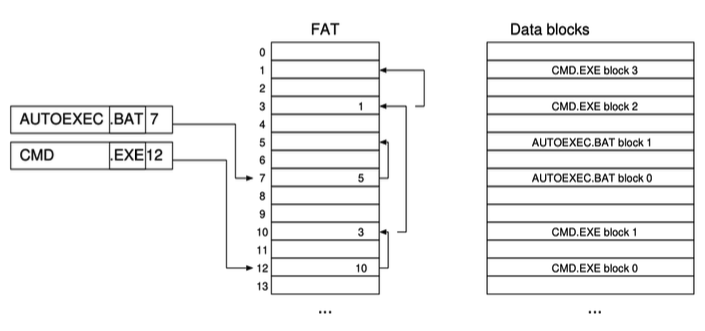
\includegraphics[width=0.9\linewidth]{fat.png}
\end{center}

For naming, the FAT system uses the filename and the extension. It then remembers the first block of that file. The file allocation table itself works like a linked list of blocks, where at the end of each block there is a pointer to the next block. To allocate new space, we simply need to scan the table. This can lead to very poor locality (fragmentation).

\subsubsection{The Berkeley Fast Filing System}

\begin{center}
	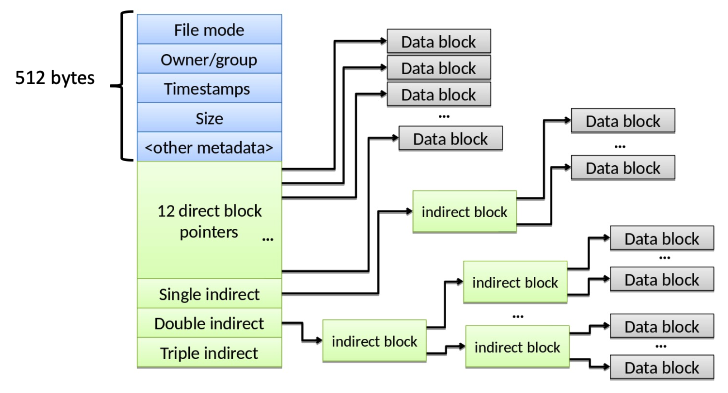
\includegraphics[width=0.8\linewidth]{bffs.png}
\end{center}

This system uses an index node (inode) for each file in the file system. The inode consists of the metadata and block pointers (or data directly if it fits). To allocate blocks it uses a bitmap indicating if a block is free or not. \medskip

Block groups are continuous subset of disk track  where related inodes, directories, free space map and file data blocks are gathered together. A superblock then holds all the informations about the overall layout and where the block groups are.

\subsubsection{Windows NTFS}

NTFS treats everything as a file, e.g. files system and file metadata. The master file table contains file entries for each file and is itself a file with the very first entry in the table. A MFT entry consists of metadata and a list of variable length attributes. One attribute is all the names for a file. If the data is small enough, it gets stored as part of the attributes, else it is stored in an extent. If works very similar to Berkeley FFS.

\begin{center}
	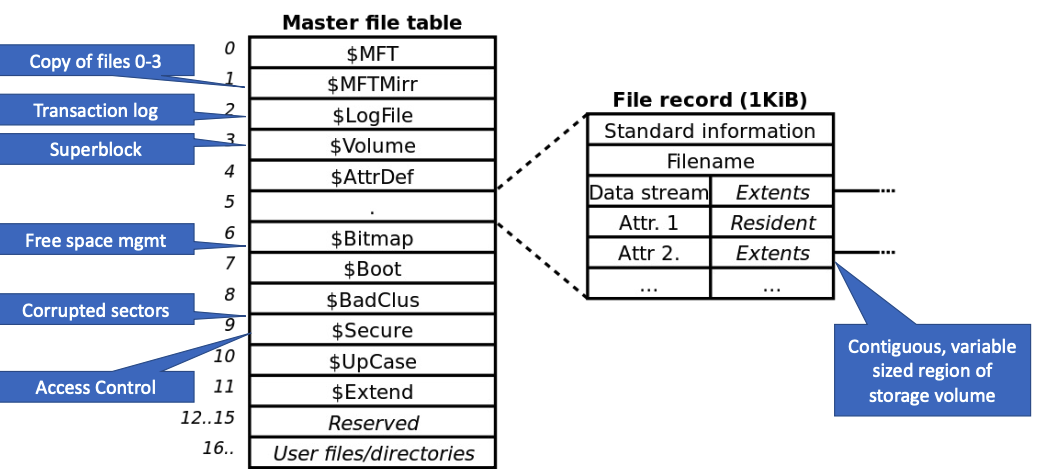
\includegraphics[width=\linewidth]{ntfs.png}
\end{center}

In NFTS file descriptors are basically pointers to extents. Additionally there are basic file descriptors.
